\documentclass[paper = a4, 12pt, oneside]{scrbook}
\usepackage{pre_style}
% \usepackage{pre_math}

% Bibliography
\usepackage[backend=biber,style=apa, sorting = nyvt,citestyle=authoryear]{biblatex}
% Add square brackets around the citation
\DeclareCiteCommand{\cite}
  {\usebibmacro{prenote}}
  {\mkbibbrackets{\usebibmacro{citeindex}\usebibmacro{cite}}}
  {\multicitedelim}
  {\usebibmacro{postnote}}

\addbibresource{bib.bib} % Import bibliography file


\usepackage[acronym,automake]{glossaries}
\makeglossaries 
    \newacronym{cmp}{CMP}{Condensed Matter physics}
    \newacronym{afm}{AFM}{Atomic Force Microscopy}
    \newacronym{moke}{MOKE}{Magneto-Optical Kerr Effect}
    \newacronym{xrd}{XRD}{X-Ray Diffraction}
    \newacronym{mo}{MO}{Magneto-Optical}
    \newacronym{si}{SI}{Supplementary Information}
    \newacronym{ree}{REE}{Rare Rarth Element}
    \newacronym{tm}{TM}{Transition Metal}
    \newacronym{edx}{EDX}{Energy-Dispersive X-ray spectroscopy}
    \newacronym{sem}{SEM}{Scanning Electron Microscopy}
    \newacronym{mfm}{MFM}{Magnetic Force Microscopy}
    \newacronym{mzm}{MZM}{Majorana Zero Mode}
    \newacronym{cqed}{cQED}{circuit Quantum ElectroDynamics}
    \newacronym{qed}{QED}{Quantum ElectroDynamics}
    \newacronym{cpu}{CPU}{Central Processing Unit}
    \newacronym{qpu}{QPU}{Quantum Processing Units}
    \newacronym{bcs}{BCS}{Bardeen–Cooper–Schrieffer theory}
    \newacronym{cpw}{CPW}{Coplanar Waveguide}
    \newacronym{pcb}{PCB}{Printed Cirucit Board}
    \newacronym{cpb}{CPB}{Cooper Pair Box}
    \newacronym{rf}{RF}{Resonator Frequency}
    \newacronym{odlro}{ODLRO}{Off Diagonal Long Range Order}
    \newacronym{dc}{DC}{Direct Current Source}
    
% \begin{figure}[h]
%     \centering
%         \includegraphics[width = 13cm]{Images/}
%         \caption[Chip overview]{\textbf{Chip overview:} }
%         \label{fig:setup_qpu}
% \end{figure}

    
\begin{document}
    \begin{titlepage}
        \def \ColourPDF {Images/ku-farve.pdf}
        \def \TitlePDF   {Images/ku-en.pdf}
    \begin{center}
        \AddToShipoutPicture*{\put(0,0){\includegraphics*[viewport=0 0 700 600]{\ColourPDF}}}
        \AddToShipoutPicture*{\put(0,602){\includegraphics*[viewport=0 600 700 1600]{\ColourPDF}}}
        \AddToShipoutPicture*{\put(0,0){\includegraphics*{\TitlePDF}}}
    \vspace*{9cm}
        \Huge
        Fluxonium


    \vspace{1.cm}
        \vfill
        \Large
        Amalie Terese Jiao Paulsen
        \\
        \large
        Supervisor: 
        \\
        Morten Kjeargaard
        \\
        \vspace{0.8cm}
        \today
        \large{\\ Number of \\
                pages: ???  \\ 
                figures: ??? \\
                characters: ???}
        
    \end{center}
\end{titlepage}
    \pagenumbering{roman}
        \pdfbookmark[1]{Abstract}{Abstract}
\chapter*{Abstract}

Here goes the Abstract: 

Theoretical part of the use of fluxonium circuit as a qubit. 
SC circuits is promising. 
Fluxonium is especially good because: 
In this piece we will write the theory of the fluxonium, simulate the energies and talk about the different parameters. 
        \pdfbookmark[1]{Acknowledgements}{acknowledgements}
\chapter*{Acknowledgements}



% A huge appreciation is expressed to my fantastic supervisors: Emmanuelle Jal and Marcel Hennes who have devoted many hours to help me within every area i possible needed it. Further thanks is given to Renaud Delaunay who has designed and build the \acrshort{moke} and magnetron located at the \acrshort{lcpmr}. Emmanuelle and Marcel have provided invaluable assistance regarding the whole internship and it would not have been the same without their help and good company. I owe them all a huge thanks.
        \setcounter{tocdepth}{2} % <-- 2 includes up to subsections in the ToC
        \setcounter{secnumdepth}{2} % <-- 2 numbers up to subsubsections
        \tableofcontents 
        \listoffigures
        \listoftables
        \printglossary[type=\acronymtype]
    \pagenumbering{arabic}
        \part{Why is Fluxonium so interesting?}\label{part:I}
            \pdfbookmark[1]{Introduction}{introduction}
\chapter{Introduction}

Why do we want to fabricate fluxonium instead of transmon qubits? 
insensitive to charge offset \Cite{Manucharyan2009}. The charges which are being accumulated in the josephson junction (can shift the energy levels + decoherence time).

            \pdfbookmark[1]{Thesis Outline}{outline}
\chapter{Outline}

This small "theoretical" paper is 1 out of 3 which in the end, will aid the theoretical part of my masters thesis. The paper is organized as the following: In the background section a brief introduction to superconductivity and BCS theory is found. This is used to describe cooper pairs and the Josephson tunnel junction. Then we build up a formalism to describe superconducting circuits using analytical mechanics and electrodynamics as well as the quantization of these. Based on this, we derive an expression for the Hamiltonian in order to find eigen energies and eigen values of the Fluxonium circuit. In the simulation section the energy levels of Fluxonium is solved numerically  in the flux basis using python. The simulation is made with sliders which can change the different parameters in order to to find the optimal theoretical values for a Fluxonium qubit. 
\\
The aim of this project is to numerically solve the energy levels of a Fluxonium circuit in order to theoretically find the optimal values of the circuit to use as the 2 defined state used as the Fluxonium qubit. 
\\
Introduce how the paper is organized and that you used python in order to simulate the eigen energies and wavefunctions of the qubit Hamiltonian
        \part{Background - The building blocks of superconducting qubits}\label{part:II}
            \pdfbookmark[1]{Background_introduction}{background_introduction}
% \chapter{Background - The building blocks of superconducting qubits}\label{chap:background_introduction}
\begin{figure}[h]
    \centering
        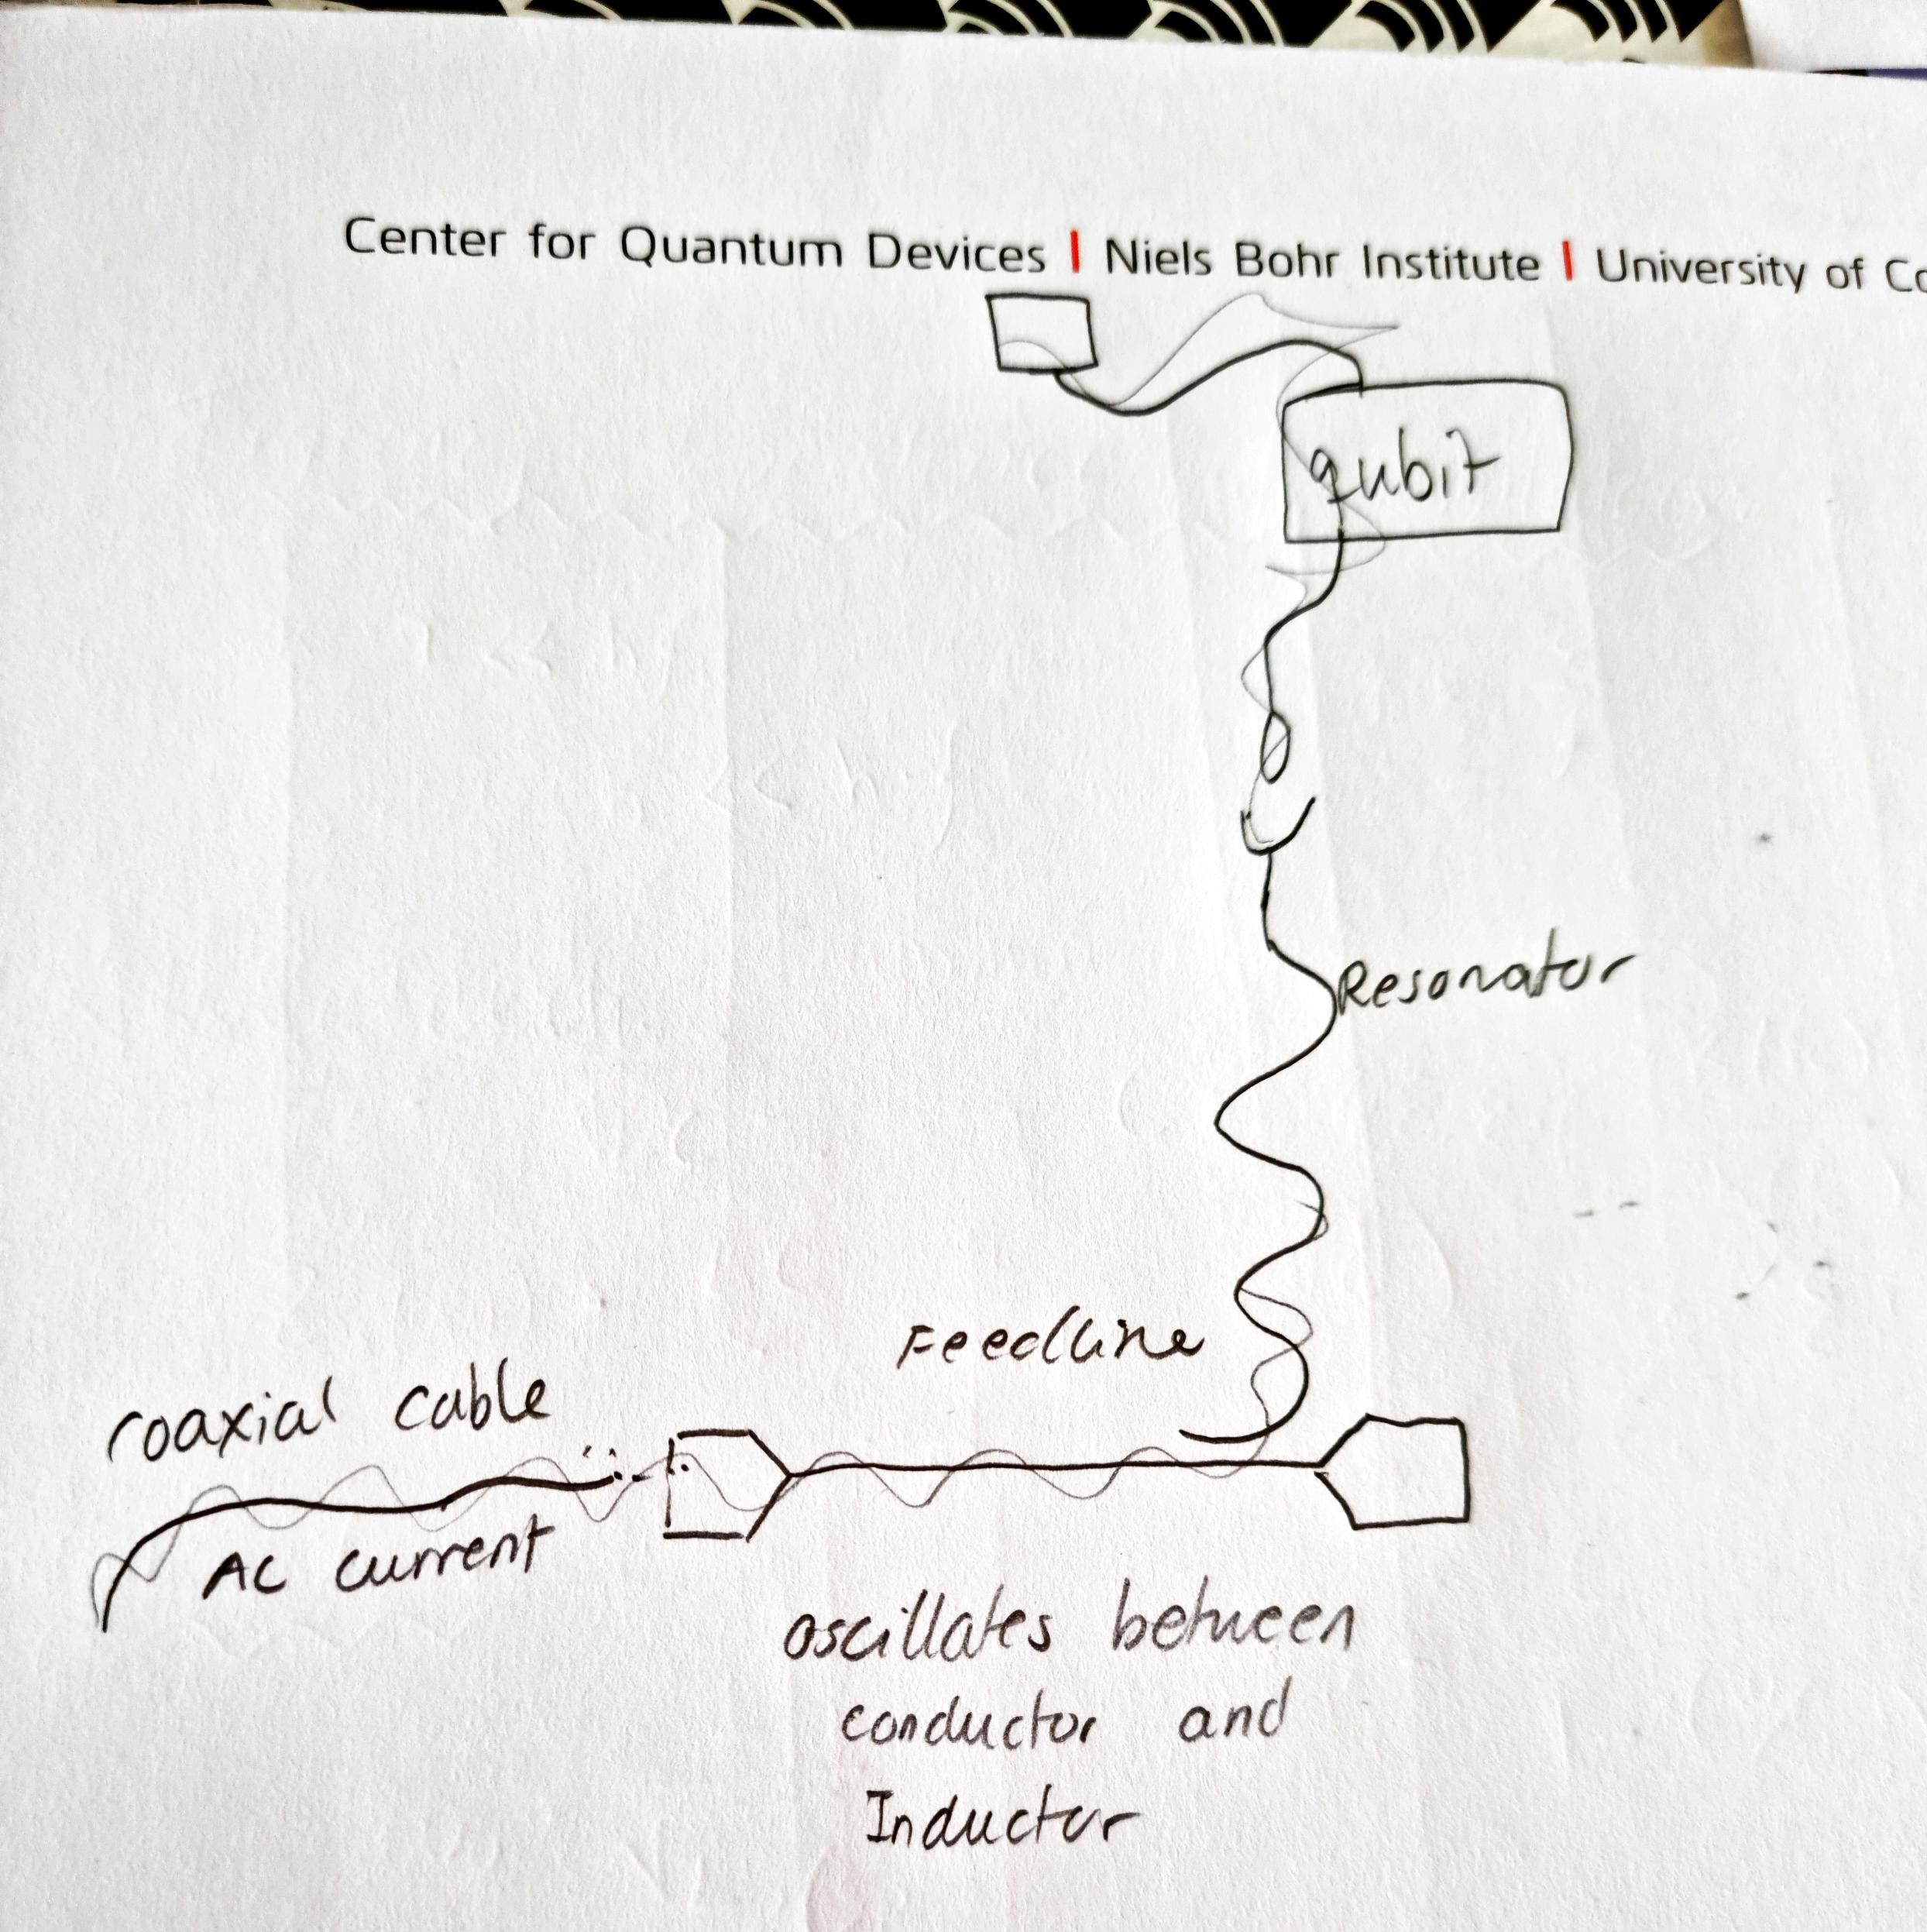
\includegraphics[width = 13cm]{Images/picture_of_setup_qpu copy.png}
        \caption[Chip overview]{\textbf{Chip overview:} This is an overview of the whole chip with the feedline, resonators and the qubits from a top view (A) and from the side view (B).}
        \label{fig:setup_qpu}
\end{figure}
%  The setup
A quantum processing unit, \acrshort{qpu}, is the heart of any quantum computer technology just like the central processing unit, \acrshort{cpu}, is of a classical computer. The fundamental building blocks of superconducting QPU design consists of superconducting transmission lines, coplanar waveguide resonators, and Josephson junctions. These components, interconnected with precision, form the cornerstone of quantum circuits that can be combined in tons of different ways to build a \acrshort{qpu} using superconducting circuits. The fig. \ref{fig:setup_qpu} is the picture of what a general model of a \acrshort{qpu} utilizing fluxonium, superconducting qubit, looks like. The coaxial cables are connected to a transmission which is capacitively coupled to a resonator connected to the qubit. The qubit is also connected to a source (typically a direct current, \acrshort{dc}, source) (called the drive line?). Each component in the circuit and each intersection between the components are described by a lot of different physics. This section aim to build a foundation for understanding some of the physics behind a fluxonium circuit. Superconducting circuits for quantum computing is a very big field utilizing many different aspects of physics, chemistry and computer science however we only briefly glance upon a few out of many interesting subareas.  
\\
% The different components we need to understand
The physics we need to take into account already start with the standard coaxial cable as the impedance needs to be matched throughout the system for eliminating reflections and power loss \cite{Pozar2012}. These happens in the interface between the coaxial cable and the feedline or the feedline and the resonator. For this we need to understand how the electromagnetic waves behave in different media and with different boundary conditions as well as how to calculate the right physical properties. It's also essential to know what types of losses can be and how we can avoid them. This field of physics is often called waveguide quantum electrodynamics. 
\\
As we are working with superconducting circuits, we also is interested in how superconductivity is obtained in different materials and what criteria for the surroundings should be present for getting the optimal environment for our qubits. 
\\
It is crucial to understand some aspects of electrical engineering and how the different components work not only from a physics perspective, but also what the role of the different components are in a circuitry. Of course we also need the knowledge we have from condensed matter physics to describe the non-linear Josephson element which are the key element for all superconducting qubits circuits.
\\
People often associate cavity QED in quantum optics with the model for the qubit in the system seen in fig.???. In this comparison, the resonators carries only the specific engineered frequencies (not sure this is why) and can be thought of as the cavity. The qubit is the 2 level system and the electromagnetic wave guided trough the system is the wave. Therefore we also take a short look into the quantum optics to describe the interaction between our 2 level system qubit and the microwave which controls it.
\\
% What is discussed in this section
In the background section we go through the theory for making the resonators, then the JJ, then the array of JJ and we talk about how to put these components together to form superconducting qubits mentioning the physics behind superconducting qubits heroff the transmon qubits, flux qubits and fluxonium. We end the chapter by discussing different advantages in the Fluxonium community up to now (this will also serve as an introduction to the simulation part.)

            \pdfbookmark[1]{resonators}{resonators}
\chapter{Resonators}\label{chap:Electromagnetic waves}
    The coaxial cables are made of a conducting wire surrounded by an insulating layer which is then surrounded by a conducting shield \cite{Griffiths2018}. This gives a 1D transmission line with boundaries allowing only a monochromatic wave to pass \cite{Schuster2007}. An electromagnetic wave in a coaxial cable has as standard an impedance of 50 Ohm\cite{Griffiths2018}. The coaxial cable is connected to a feedline which is again capacitively coupled to some resonators. 
    \section{Transmission line resonator modeled as a LC circuit}
        \begin{figure} [h]
            \centering
                \includegraphics[width = 13cm]{Images/Transmission line resonator modeled as a LC circuit.png}
                \caption[Transmission line resonator modled as a LC Circuit]{\textbf{Transmission line resonator modled as a LC Circuit:} Here}
                \label{LC circuit}
        \end{figure}
    \section{Transmission line resonator capacitively coupled to}
        \begin{figure} [h]
            \centering
                \includegraphics[width = 13cm]{Images/Transmission line resonator capacitively coupled to a feedline.png}
                \caption[Transmission line resonator capacitively coupled to a feedline]{\textbf{Transmission line resonator capacitively coupled to a feedline:} Here}
                \label{LC circuit capacitively coupled to feedline}
        \end{figure}
    Coplanar waveguide is a special type of transmission line resonators very commonly used in superconducting circuits for quantum building quantum computers (use some references here.) In the following section, we will describe what specifically type of coplanar waveguide (lambda 2 and lambda4 resonators (open and shunt)), how the electric field is distributed, how their geometry is, how they are described (mathematically), what materials are used and why (aluminium, because they are superconducting), 
    \section{Coplanar waveguide cavities modeled as LC circutis?}
    \begin{figure} [h]
        \centering
            \includegraphics[width=13cm]{Images/2D_Chip_dim.png}
            \caption[Coplaner waveguide]{\textbf{Coplanar waveguide:} This is a model of a CPW feedline capacitively coupled to a CPW resonator. The left side is a picture of the top view of the whole chip. The right is a picture of the cross section taken at the black line found in the top view. The grey regions represents a superconducting film and the blue our substrate. The superconducting film is etched to create the resonators and the feedline. They both have width (a) and and distance (s) to the rest of the superconducting film for impedance matching.}
        \label{fig:2D_chip_dim}
    \end{figure}
    Feedlines and resonators have many similarities but are used very differently how??. While the feedline allow voltages and currents with many different magnitudes and phases to be transmitted through, the resonators only allows waves of specific frequencies to live inside it \cite{Pozar2012}. Fig. \ref{fig:2D_chip_dim} shows us the geometry of the feedline and the resonator. The left side is a top view of the whole chip containing a feedline and a resonator while the right side is a cross sectional view which highlight the device geometries. The cross section is taken at the black line shown in the top view. The grey regions represents a superconducting film and the blue our substrate. In this thesis, we will use Aluminium (Al) as our superconducting film and Silicon (Si) as our substrate. The superconducting film is etched to create the resonators and the feedline. They both have width (a) and and distance (s) to the rest of the superconducting film for impedance matching. 
    \newline
    \newline
    The device geometry and the dielectric properties of the resonators play a great role on the frequency. We are mainly working with $\lambda / 2$ and $\lambda / 4$ resonators \cite{Pozar2012}.  These two types of resonators can be engineered as a short- or open circuited as seen in fig. \ref{fig:lambda2_and_lambda4}. The frequency of the lambda and lambda4 resonator is given by \cite{Goppl2008}: 
    \begin{figure}
        \centering
            \includegraphics[width=10cm]{Images/lambda2 and lambda4 resonators_total.png}
            \caption[$\lambda$2 and $\lambda$4 resonators]{\textbf{$\lambda$2 and $\lambda$4 resonators:} This is a picture of the $\lambda$2 and $\lambda$4 resonators. The $\lambda$2 resonator are short in both ends.the $\lambda$4 has 1 end shorted and 1 end open}
        \label{fig:lambda2_and_lambda4}
    \end{figure}
    \begin{equation}
        \begin{aligned}
            w_{0,\lambda 2} &= \frac{c}{\sqrt{\epsilon_{\mathrm{eff}}}} \frac{1}{2 l} \\
            w_{0,\lambda 4} &= \frac{c}{\sqrt{\epsilon_{\mathrm{eff}}}} \frac{1}{4 l}
        \end{aligned}
    \end{equation}
    Where $2l = \lambda_{2,0}$ and $4l = \lambda_{4,0}$ is the wavelength of the resonator mode and the $\epsilon_{\mathrm{eff}}$ is the effective dielectric constant given by. 
    \begin{equation}
        \epsilon_{\mathrm{eff}}=\frac{1+\epsilon_{\mathrm{r}} \widetilde{K}}{1+\widetilde{K}}
    \end{equation}
    And K(k) and K(k') are elliptical integrals given by: 
    \begin{equation}
        \begin{gathered}
            \widetilde{K}=\frac{K\left(k^{\prime}\right) K\left(k_3\right)}{K(k) K\left(k_3^{\prime}\right)} \\
            k=\frac{a}{a+s} \\
            k_3=\frac{\tanh \left(\frac{\pi a}{4 h}\right)}{\tanh \left(\frac{\pi (a+s)}{4 h}\right)} \\
            k^{\prime}=\sqrt{1-k^2} \\
            k_3^{\prime}=\sqrt{1-k_3^2}
            \end{gathered}
    \end{equation}
	The frequency of both lambda4 and lambda2 resonators are highly dependent on the device geometry and the length of the resonators. Keeping the same geometries for all resonators in our system, we can vary their frequency by simply changing the length. 
    
    
    
    \subsection{Impedance}
        We can express the dissipation of our system as an impedance. At our typical operating temperature for superconducting systems ($T<T_c$) the DC resistance vanish shown by the meissner effect in the next section. However, there are a small non-zero contribution to the impedance due to the AC electric fields \cite{Zmuidzinas2012}. The impedance of the coaxial cable has to match the one of feedline and the resonator in order to eliminate as many unwanted reflections as possible as this will lead to power loss \cite{Pozar2012}. When the impedance matches perfectly, you will maximize the power transferred between each component. However, calculating impedance is strongly geometrical dependent. We can model both the feedline and the resonator as a LC lumped element.
        % Let's get something in the clear: 
        % \begin{itemize}
        %     \item $Z_{0}$ is the impedance from the the cables and is 50 ohms
        %     \item $Z_{r}$ = impedance inside the resonator?
        %     \item $Z_{fl}$ = impedance inside the feedline
        % \end{itemize}
        We always assume, that the impedance going from the cables to our system is $50 \Omega$ For a system which is in perfect impedance matching throughout the system, we use $Z_{0}$  for all of the values above. We can express the impedene of our resonators as \cite{Pozar2012}.
        \begin{equation}
            Z_{0} = \sqrt{\frac{L}{C}}
        \end{equation}
        Where L is the total inductance and C is the total capacitance of the resonator. 
        \begin{equation} 
            \begin{aligned}
                L &= \frac{2}{\pi^{2} n^{2}} L_{\ell} l \\
                C &=\frac{1}{2} C_{\ell} \ell
            \end{aligned}
        \end{equation}
        The $C_{\ell}$ is the capacitance (of what? the total capacitance or the capacitance of the coupling?) and depend on???
        It is given by the formula: 
        \begin{equation}
            C_{\ell}=4 \varepsilon_0 \varepsilon_{e f f} \frac{K(k)}{K\left(k^{\prime}\right)}
        \end{equation}
        l is the length of the resonator and $L_{l}$ is the total inductance. The inductance depend highly on the geometry and material properties at a certain temperature. It is given by 2 terms \cite{Schuster2007}:
        \begin{equation}
            \begin{gathered}
                L_m=\frac{\mu_0}{4} \frac{K\left(k^{\prime}\right)}{K(k)} \\
                L_k=\mu_0 \frac{\lambda_L^2}{W t} g(s, a, t) \\
                L_{\ell} = L_{m} + L_{k}
            \end{gathered}
        \end{equation}
        $L_m$ is the inductance stored in the feedline. The $L_k$ is the kinetic inductance and is due to the fact that electrons itself is creating a small inductance when moving \cite{Schuster2007}. $\mu_{0}$ is the Vacuum permeability and g is a geometrical function given by: 
        \begin{equation}
            g(s, a, t)=\frac{1}{2 k^2 K(k)^2}\left(-\ln \left(\frac{t}{4 a}\right)+\frac{2(a+s)}{(a+2 s)} \ln \left(\frac{s}{a+s}\right)-\frac{a}{(a+2 s)} \ln \left(\frac{t}{4(a+2 s)}\right)\right)
        \end{equation}
        Note that since our resonators has the geometry as a snake, there is also a contribution from the geometry in the inductance which is added, however this is not taken into account in this work. This shows, that the impedence is very sensitive to the device geometry. In order to match the impedance, we need to design the resonators and feedline to $ 50 \Omega$. 

    


        \subsection{Quality factors}
        The quality factor is a measure of how much energy is stored over how much energy is stored pr. time. We can use the Quality factor to say something about how lossy our circuit is in terms of photons. Many factors are at play when talking about the losses, conductor loss, dielectric loss, radiation loss. Often the losses occur due to the way of fabrication and there is no way to be sure what your $Q_factor$ are before fabrication. However, there are some equations relating the Q factor to the different components which are used for fitting the data later on. Systems like the one in fig. \ref{fig:2D_chip_dim} where a coplanar waveguide resoantor is capacitively coupled to a feedline, there are 2 characteristic qualitifactors to take into account. The intrinsic or unloaded quality factor, $Q_i$, and the external or the loaded quality factor, $Q_e$. The two quality factors have the following relation:
        \begin{equation}
            \frac{1}{Q_{T}} = \frac{1}{Q_{c}} + \frac{1}{Q_{i}} 
        \end{equation}
        The unloaded quality factor (that is how lossy the resonator is out of context in a coupled circuit), can be expressed by: 
        \begin{equation}
            Q_i=\omega_0 \frac{W_m+W_e}{P_{\text {loss }}}=\omega_0 R C=\frac{R}{\omega_0 L}
        \end{equation}
        The external quality factor highly depend on how strongly coupled the resonator is to the feedline and is described by: (FIND OUT WHAT THE x IS!)
        \begin{equation}
            \begin{aligned}
                Q_c &= \omega_0 C_T Z_x=\sqrt{\frac{C_T}{L}} \frac{2}{\omega_0^2 C_c^2 Z_0}\\    
            \end{aligned} 
        \end{equation}\label{eq:Qc}
        Even though the total capacitance is divided into two parts, we can find the total capacitance using the following relation: 
        \begin{equation}
            C_{T} = C + C_{c} = > C_{c} = C_{T} - C
        \end{equation}
        Where C is the unloaded resonator capacitance and $C_c$ is the capacitance due to coupling to the feedline. The coupling can be made smaller by making the gap larger (makes sense, but I  need to see it in the picture). 
        \\
        Depending on the fabrication and thereby the Q-factor, the electromagnetic wave will be scattered, transmitted and reflected with different ratios described by the scattering matrix: S



        \subsection{Looses in superconducting resonators}
        Many things can effect the quality factor. Since we can interpret the quality factor as a measure of how much dissipation there are inside the resonator, we typically say that "loss" in a superconducting resonator is the loss of photons. In the following we briefly mention some of the reasons for loss.
        \\
        Loss can occur as radiation into the free space \cite{Zmuidzinas2012}. 
        Losses are due to geometrical factors or defects occurring in the fabrication process. Why are we t in losses? changes the $Q_i$?
        \\
        Two level system loss
        \\	
        Magnetic vortices loss 
        \\
        Loss uncertainty 
        \\
        Radiation loss
        \\
        All these losses can lead to a change in the Q-factor and the scattering, transmission and reflection will also make our system non-ideal which results in transmission and  reflection and even phase change, amplitude changes and so on. 



    \subsection{Scattering Matrix}
        The scattering matrix give a description of how an incident wave is transmitted, reflected and scattered \cite{Pozar2012}. In this context, the matrix is used to relate the incident voltage wave with the reflected when using a 2 port network (from a VNA) connected to each end of the feedline. We are mostly interested in the transmission which takes the form \cite{Khalil2012}.  
        \begin{equation}
            S_{21} \equiv \frac{V_{out}}{V_{in}}
        \end{equation}
        Where $V_{in}$ is the voltage going into the feedline and $V_{out}$ is the voltage going out of the feedline. For a hanging resonator like the one in fig. \ref{fig:2D_chip_dim} this will give a dip like in fig. \ref{fig:resonator_dip}- 
        \begin{figure}[h]
            \centering
            \includegraphics[width = 10 cm]{Images/Resonator_dip.png}
            \caption[Characteristics of resonator dip]{\textbf{Characteristics of resonator dip:} This is a picture of how a resonator dip can look like.}
        \label{fig:resonator_dip}
        \end{figure}
        The transmitted voltage through the feedline can be fitted by a lorentzian taken the form \cite{Zmuidzinas2012}:
        \begin{equation}
            S_{21}(\omega) = 1 - \frac{\frac{Q_{l,r}}{Q_c}}{1+i2Q_{l,r}(\frac{\omega-\omega_0}{\omega_0})}
        \end{equation}
        Where $Q_{l,r}$ is the overall quality factor of the resonator, $Q_c$ is the coupling quality factor of the resonator and $\omega_0$ the resonator resonance frequency. This fitting model relates the Quality factors mentioned before and we use it to extract the $Q_i$ and $Q_c$ of our resonators. 
        % In order to focus on the central dip and not take the tail of the lorentzian into account, we find the full width at half maximum ($\delta_f$) which corresponds to around 3dB from the $S_{21}$ min  \cite{Barlow1989}.
        % \begin{equation}
        %     L = 10\cdot Log_{10}(\frac{P}{P_0}), \frac{P}{P_0} = 0.5 \Rightarrow L = 10\cdot Log_{10}(0.5) \approx 3 dB
        % \end{equation}
        % We will take this as the width of the dip. We can then express the relationship between the Q factors and the scattering matrix as:
        % Using this formula, we can write the unloaded Q_factor = Q_e as: 
        % \begin{equation}
        %     Q = \frac{\omega_0}{\Delta f}
        % \end{equation}
        \begin{equation}
            \begin{gathered}
                Q_c=\frac{Q_{l,r}}{1-\min \left(\left|S_{21}\right|\right)} \\
                Q_i=\frac{Q_{l,r}}{\min \left(\left|S_{21}\right|\right)}
            \end{gathered}
        \end{equation}
        Usually the $Q_c$ is close to the value found using the eq. \ref{eq:Qc} and is in the order of $e5$. You want as high $Q_i$ as possible we typically have in the order of  $e6$ but there have been shown $Q_i$ factors in the order of $e8$ for high powers \cite{Crowley2023b}. However, working with superconducting resonators, you typically want to see what your $Q_i$ is in the single photon regime as it is also the regime where we want to operate our qubit. In order to measure if we are in the single photon regime, we want to write a relation between the photon number and the power we send out. 


    \subsection{Photon number}
        We want to be in the single photon regime (in order to mimic the one of the qubit which is also just taking 1 photon in and 1 out). However, we can only estimate the number of photons \cite{Bruno2015}: 
        \begin{equation}
            \left\langle n_{p h}\right\rangle=\frac{2}{\hbar \omega_0^2} \frac{Q_{l,r}^2}{Q_c} P_{i n}
        \end{equation}
        Where $P_{in}$ is the number of photons going into the feedline and $\omega_0$ is the frequency of our resonator. We need to remember, that the current going from the VNA is the not the current going through our feedline as we have coupled a lot of different attenuators and amplifiers. These need to be taken into account. 
        

    \subsection{Quantization of the LC harmonic oscillator}
    From schuster p. 60. since we are working with QM, we want to describe the LC circuit quantum mechanically. The quantization gives a hamiltonian: 
    also blais p. 5
    \begin{equation}
        H = \hbar \omega (a^{\dagger} a + \frac{1}{2})
    \end{equation} 
    The energy of an inductor, the energy of a capacitor (as we should use it in the next section. )
            \pdfbookmark[1]{jj}{jj}
\chapter{Josephson junctions}\label{chap:jj}



\section{Superconductivity}
    \begin{figure}
        \centering
        \includegraphics[width = 13cm]{Images/critical field.png}
        \caption[Type 1 and type 2 superconductor]{\textbf{Type 1 and type 2 superconductor:} A) Type 1 superconductor. $H_c$ is the critical field where the magnetization gets destroyed. instantaneously. B) Type 2 superconductor have two critical fields, $H_{c1}$ and $H_{c2}$. At $H_{c1}$, some flux-lines start to be able to enter the superconductor. At $H_{c2}$, the superconductivity is destroyed and the superconductor don't produce a magnetization anymore. C) and D) the critical temperature $T_c$ as a function of the external magnetic field applied.}
        \label{fig:type1and2}
    \end{figure}
    A superconductor is a material in which you can prove the Meissner–Ochsenfeld effect below a critical temperature, $T_c$, or at very high pressures. The Meissner effect is a property of thermal equilibrium and states that a weak external magnetic field will be expelled by a superconductor below $T_c$ independently of how it was cooled down. In order for the superconductor to repel the small external magnetic field, $\Vec{B}_{ext}$, it must produce an equal but opposite magnetization \cite{Annett2004}: 
    \begin{equation}
        \Vec{B}_{ext}=\mu_0 (\Vec{H}_{ext} + \Vec{M}) = 0 \Leftrightarrow \Vec{H}_{ext} = - \Vec{M}
    \end{equation}
    The magnetic susceptibility is then given by: 
    \begin{equation}
        \chi=\left.\frac{d M}{d H}\right|_{\lim_{H\to 0}}= -1
    \end{equation}
    This tells us the superconductor is a diamagnet and since it completely repels the external field, it is said to be a perfect diamagnet. However, this is only true for small external fields. When the strength of the field increases, two possible things can happen dependent on, if the superconductor is type 1 or type 2. A type 1 superconductor will repel the external magnetic field until a critical field, $H_{c}$. At this field, the superconductivity is abruptly destroyed and the magnetization, $\Vec{M}$ goes to 0 instantaneously as seen in fig. \ref{fig:type1and2} A). A type 2 superconductor exhibit a change in behavior at two critical fields, $H_{c1}$ and $H_{c2}$. At $H_{c1}$, some flux-lines start to be able to enter the superconductor. The amount of flux-lines which can enter, will increase linearly between $H_{c1}$ and $H_{c2}$ as a function of $H$. At $H_{c2}$, the superconductivity is destroyed and the superconductor don't produce a magnetization anymore as seen in fig. \ref{fig:type1and2} B. The critical fields for which both type 1 and type 2 superconductors change behavior, is itself a function on temperature. This is seen in fig. \ref{fig:type1and2} B) and C). At $T_c$ the superconductors undergo a 2nd order phase transition from a "superconductor" to a "normal metal". Since we are only interested in the superconducting properties, we will from now on only assume temperatures below $T_c$. 
    \newline
    \newline
    Besides, from the magnetic properties of superconductors, they are also shown to posses persistent current meaning it can carry a current without an external energy source. The persistent current is due to the fact, that superconductors exhibit zero resistivity, $\rho = 0 $, and can therefore carry a flow of electrons without getting scattered into phonons or other electrons. The relationship between the super current density and the magnetic vector potential is given by the London equation \cite{Annett2004}:
    \begin{equation}
        \Vec{j}_s=-\frac{n_s e^2}{m_e} \Vec{A}
    \end{equation}
    The current running in superconductors is due to cooper pairs which are pairs of electrons. The cooper pairs and the critical temperature can be described by the Bardeen–Cooper–Schrieffer theory, \acrshort{bcs} theory. The \acrshort{bcs} theory is a microscopic quantum theory of superconductivity and is described in the following section in order to better understand why electrons forms cooper pairs and what conditions should be fulfilled in doing so. 
  
    \subsection{Mean field BCS theory and cooper pairs}
         The formation of cooper pairs is due to an attractive potential between 2 electrons close to the Fermi surface. Electrons interact via a phonon where the effective potential is given by \cite{Annett2004}: 
          \begin{equation}
            V_{\mathrm{eff}}{q}, \omega)=\left|g_{\mathrm{eff}}\right|^2 \frac{1}{\omega^2-\omega_D^2}
        \end{equation}
        If $|\omega < \omega_D|$, the effective potential is attractive. Therefore, it is only electrons which have energies within $\varepsilon_f \pm \hbar \omega_D$ which participate in forming cooper pairs. Assuming all states up to the fermi wave vector, $k_f$, is filled. Adding 2 electrons within $\varepsilon_f +\hbar \omega_D$ will create a cooper pair. The 2 particle wave function is anti symmetric and can be divided into two parts, a spacial- and a spin wave function: 
        \begin{equation}
            \Psi(r_1,r_2,\sigma_1,\sigma_2) = e^{i\Vec{k}\Vec{r}} \varphi(r_1-r_2) \phi^{spin}_{\sigma_1,\sigma_2}
        \end{equation}
        Due to anti symmetry of Fermions, we know that the position and spin wave function should have opposite symmetry. The lowest energetic configuration is when the cooper pairs have opposite k-vector and therefore $\Vec{k}=0$. Further, the position wave function: $\varphi\left(\mathbf{r}_1-\mathbf{r}_2\right) = + \varphi\left(\mathbf{r}_2-\mathbf{r}_1\right)$ is an even function. Therefore, $\phi^{spin}_{\sigma_1,\sigma_2} = \frac{1}{\sqrt{2} }|\uparrow \downarrow \rangle - |\downarrow \uparrow \rangle $ is an uneven function and it turns out that it is in a singlet state \cite{Annett2004}.
        \newline
        \newline
        The  Hamiltonian for describing the electron-electron interaction for opposite spin, $\sigma_1=-\sigma_2$,  and opposite k vector, $k_1=-k_2$ is given by\cite{Annett2004}: 
        \begin{equation}\label{Hamiltonian_BCS}
            \hat{H}=\sum_{\mathbf{k}, \sigma} (\varepsilon_{\mathbf{k}}-\mu) c_{\mathbf{k} \sigma}^{\dagger} c_{\mathbf{k} \sigma}-\left|g_{eff}\right|^2 \sum_{\mathbf{k} \mathbf{k'}} c_{\mathbf{k}_{\uparrow}}^{\dagger} c_{-\mathbf{k}_{\downarrow}}^{\dagger} c_{\mathbf{k'}_{\downarrow}} c_{\mathbf{k'}_{\uparrow}} 
        \end{equation}
        The first term is the self energy of an electron and the second term is the electron-electron interaction. The $c$ and $c^{\dagger}$ is the operators which change the occupation number of the Fock space.
        \begin{equation}
            c^{\dagger}|0\rangle = |1\rangle, c |1\rangle = |0 \rangle
        \end{equation}
        We use a mean field approximation and the Bogoliubov-Valentin transformation and rewrite the Hamiltonian as: 
        \begin{equation}
        \hat{H}_{MF}= \sum_{\mathbf{k} ,\sigma} (\varepsilon_{\mathbf{k}}-\mu) c_{\mathbf{k} \sigma}^{\dagger} c_{\mathbf{k} \sigma}-\left|g_{eff} \right|^2 \sum_{\mathbf{k} \mathbf{k'}} \left(\langle c_{\mathbf{k_{\uparrow}}}^{\dagger} c_{-\mathbf{k} \downarrow}^{\dagger}\rangle c_{-\mathbf{k}^{\prime}_{\downarrow} }c_{\mathbf{k}^{\prime}_{\uparrow}} + c_{\mathbf{k}_{\uparrow}}^{\dagger} c_{-\mathbf{k}_{\downarrow}}^{\dagger} \langle c_{-\mathbf{k'}_{\downarrow}} c_{\mathbf{k'_{\uparrow}}} \rangle \right)
        \end{equation}
        Due to symmetry of our occupation number operators, this  can be rewritten into: 
        \begin{equation}
            \hat{H}_{MF}=\sum_{\mathbf{k} \sigma}\left(\varepsilon_{\mathbf{k}}-\mu\right) c_{\mathbf{k} \sigma}^{\dagger} c_{\mathbf{k} \sigma}-\sum_{\mathbf{k}}\left(\Delta^* c_{-\mathbf{k} \downarrow} c_{\mathbf{k} \uparrow}+\Delta c_{\mathbf{k} \uparrow}^{\dagger} c_{-\mathbf{k} \downarrow}^{\dagger}\right)
        \end{equation}
        Where $\Delta$ is defined as: 
        \begin{equation}
            \Delta = \left|g_{eff} \right|^2 \sum_{\mathbf{k}} \langle c_{-\mathbf{k'}_{\downarrow}} c_{\mathbf{k'_{\uparrow}}} \rangle
        \end{equation}
        We can now write the Hamiltonian in the form of a matrix: 
        \begin{equation}
            \hat{H}_{MF}=\sum_{\mathbf{k}}\left(\begin{array}{ll}
            c_{\mathbf{k} \uparrow}^{\dagger} & c_{-\mathbf{k} \downarrow}
            \end{array}\right)\left(\begin{array}{cc}
            \varepsilon_{\mathbf{k}}-\mu & -\Delta \\
            -\Delta^* & -\left(\varepsilon_{\mathbf{k}}-\mu\right)
            \end{array}\right)\left(\begin{array}{c}
            c_{\mathbf{k} \uparrow} \\
            c_{-\mathbf{k} \downarrow}^{\dagger}
            \end{array}\right)
        \end{equation}
        The eigen energies of the square matrix is $E_k = \sqrt{(\varepsilon_k-\mu)} + |\Delta|^2$. The relationship between $\Delta$ and $E_k$ is very important as it tell us how an incoming electron into a superconductor behave and thereby the energy needed to create a cooper pair. We call $\Delta$ our order parameter and it determines if we are in the normal state (above $T_c$, $\Delta = 0$) or in the superconducting state (below $T_c$, $\Delta \neq 0$). In the superconducting state, the energy associated with adding an electron is $+E_k$. The minimum energy associated for making an excitation is $2\Delta$ which is the energy gap of the superconductor. Electrons going into the superconductor must therefore posses energy $E_k > \Delta$  which is why it can be related to the binding energy of creating a cooper pair.
        
    \subsection{Josephson tunnel junction}
        \begin{figure}
            \centering
                \includegraphics[width = 10cm]{Images/Josephson junction.png}
                \caption[Schematic drawing of a Josephson Junction]{\textbf{Schematic drawing of a Josephson junction:} The $\theta_L$ and $\theta_R$ is the phase of each superconductors. The $\psi_L$($\psi_R$) is the macroscopic wave functions describing the cooper pairs on the left(right) superconductor.}
            \label{fig:JJ}
        \end{figure}
        A Josephson junction is an electrical component consisting of 2 superconductors separated by an insulating layer as seen in \ref{fig:JJ}. The Josephson junction allows the tunneling of cooper pairs between the two superconductors through the insulating layer. This tunneling effect is called the Josephson effect. It can be described mathematically because the states of the cooper pairs on each superconductor can be described by a coherent wave function $\psi_0$ which posses  Off Diagonal Long Range Order, \acrshort{odlro}. \acrshort{odlro} can be physical interpreted as the coherent wave function describing cooper pairs (pairs of electrons) is valid even though the cooper pairs are very far away. By using the macroscopic wave function to describe the cooper pairs on each side, the hamiltonian for describing the whole system becomes: 
        \begin{equation}
        \hat{H} = 
            \begin{bmatrix}
            \frac{2eV}{2} & T \\
            T & -\frac{2eV}{2} 
            \end{bmatrix} 
        \end{equation}
        Where the $2e$ is from the charge of the 2 cooper pairs and $ \pm \frac{V}{2}$ is the voltage lifted(lower) the potential in the side. The $T$ is the transmission term which says how easily the cooper pairs are able to tunnel through the insulating layer. $T$ is dependent on the thickness and materials of the insulating layer. Inserting the Hamiltonian into the Schrodinger equation will give the following equations: 
        \begin{equation}
                \frac{d \Psi}{d t} 
            =
                \frac{1}{i \hbar}\hat{H}\Psi
            \Rightarrow
                \begin{bmatrix}
                    \frac{d \psi_L}{dt} \\
                    \frac{d \psi_R}{dt} 
                \end{bmatrix}  
            =    
                \frac{1}{i \hbar} 
                \begin{bmatrix}
                \psi_L e V + \psi_R T \\
                \psi_L T - \psi_R e V  
                \end{bmatrix}
        \end{equation}
        The current from one side to the other in the Josephson junction is given by the change in number of cooper pairs in one superconductor over time multiplied with the charge of the cooper pairs: 
        \begin{equation}
            \begin{aligned}
                I_L &= -I_R =  \frac{d|\psi_L|}{dt} 2e = 2e \left( \Dot{\psi}_L^* \psi_L + \psi_L^* \Dot{\psi_L} \right) \Rightarrow 
                \\
                I_L &= \frac{2e}{i\hbar} \left( -eV |\psi_L|^2 - \psi_R^*\psi_L + e V  |\psi_L|^2 + T \psi_L^*\psi_R \right) 
            \end{aligned}
        \end{equation}
        Using that $\psi_{L(R)} = Re(\psi_{L(R)}) + i Im(\psi_{L(R)})$ and $\psi_{L(R)}^* = Re(\psi_{L(R)}) - i Im(\psi_{L(R)})$, we obtain that only the imaginary part is left: 
        \begin{equation}
            I_L = \frac{4 e T}{\hbar} Im(\psi^*_L \psi_R)
        \end{equation}
        Assuming that the transmission, $T$, is small, we can approximate the off diagonal terms in the Hamiltonian as a small perturbation to a system with no transmission of cooper pairs, $\mathring{\Psi}$. 
        \begin{equation}
            \begin{aligned}
                 I_L &= \frac{4 e T}{\hbar} Im(\mathring{\psi}^*_L \mathring{\psi}_R) + \text{small perturbation} \\
                    \mathring{\psi}^*_L &= |\mathring{\psi}_L| e^{(i V e)/\hbar t - i\theta_L}\\
                    \mathring{\psi}_R &= |\mathring{\psi}_R| e^{(i V e)/\hbar t + i\theta_R}
            \end{aligned}
        \end{equation}
        \begin{equation} \label{eq:JJ1}
            \Rightarrow I_L = I_c sin(\Delta \theta)
        \end{equation}
        Where $\Delta \theta = \theta_R- \theta_L$ is the difference in phase between the 2 superconductors and $I_c = \frac{4 e T }{\hbar}$ is the critical current dependent on the geometry and material of the insulating layer. The critical current is the max current the copper pairs can make. Currents $I< I_L$ are dissipationless and are often referred to as a super current $I_S = I_L $.  The eq. \ref{eq:JJ1} is called the first Josephson equation and tells us that the supercurrent, $I_s$ is proportional to to the phase difference between the two superconductors. The other Josephson equation is given by: 
        \begin{equation}
            \begin{aligned}
                \frac{\partial\Delta \theta}{\partial t } &= \frac{2e}{\hbar} V(t) \\
                V(t) &= \frac{\partial \Delta \theta}{\partial t} \frac{\hbar }{2 e}
            \end{aligned}
        \end{equation}
        Which gives us a relation between the change in phase and the voltage applied. When a current runs through the Josephson junction, there will be stored an energy depended on the phase difference between the two superconductors, $\Delta \theta$. The energy is given by \cite{Krantz2019}:
        \begin{equation}
            E(\Delta \theta) = -E_J cos(\Delta \theta) 
        \end{equation}
        Where $E_J =  \frac{\Psi_0 I_c}{2 \pi}$. From now on, we will write $\Delta\theta = \phi$. 
        Some text where you end up with the hamiltonian as we show in 
        \begin{equation}
            Josephson: \quad h_{J} = E_j \cos \left(\frac{\Phi 2 \pi}{\Phi_0} \right)    \\
        \end{equation}

    \subsection{Manhattan style junction}
    Josephson junction equal SIS junction can be made in different ways. The most common is the Manhattan and the doland bridge. we will focus on the Manhattan style in this thesis
        Double angle evaporation (make drawing). 

        The relation between the resistance and the Josephson energy


            \pdfbookmark[1]{jj_array}{jj_array}
\chapter{Array of Josephson junctions}\label{chap:jj_array}

\section{Superinductance}
\section{Effective inductance}
\section{Inductive loss in Josephson junction arrays}

We want to end up with 
\begin{equation}
    E_L = \frac{E_J2?1}{N}
\end{equation}
            \pdfbookmark[1]{Super_conducting_qubits}{Super_conducting_qubits}
\chapter{Superconducting qubits}\label{chap:Super_conducting_qubits}



\section{Interaction of atoms and electromagnetic waves}
    In superconducting circuits, it is the ?? find out elements of the Josephson junction which constitute our qubits in our \acrshort{qpu} and the electromagnetic waves we use to control and manipulate the qubits. For this it is important to know what happens when they interact. Therefore, we will dig deeper into how we can describe the interaction between electromagnetic waves and the 2 level qubits using the Jaynes cummings hamiltonian. Typically the qubits are operated within the microwave-range corresponding to frequencies 
    \\
    Write what you find out in quantum optics course. 
        laser (coherent state?) interacting with a 2 level system in a cavity? is it really a cavity? ask peter. 
    \\
    A series of specific manipulations (rotations) are called gates. 
    \\
    Talk about how we use light to go around on the bloch sphere. 
    \\
    In quantum computing we want some very specific ways of manipulating out qubits (gates) which are discussed in the next section.
    
        
\section{Superconducting circuits architecture}
    A classical circuit consists of components like capacitors, inductors, and resistors. The components are referred to as branches and these are connected by wires called nodes \cite{Griffiths2018}. A closed path where each node and branch only are represented once, is called a loop. One can utilize superconducting materials in order to fabricate the circuit components. Doing so, quantum mechanic effects will be non-neglectful and should be taken into account \cite{Girvin2014}. The strategy for describing the dynamics in quantum circuits is to use analytical mechanics and electrodynamics. Then we will quantize the charge and the flux to end up with the Hamiltonian of our system \cite{Krantz2019}. We relate the magnetic flux to the phase as  $\Phi= \frac{1}{2\pi}\Phi_{0} \phi \Rightarrow \phi = \frac{\Phi 2 \pi}{\Phi_0}$. The phase can also be interpreted as the reduced flux quantum. Then the energies of the different components are: 
    \begin{equation}
        \begin{aligned}
            Capacitor:& \quad h_C  = \frac{C}{2} \Dot{\Phi}^2     \\ 
            Inductor:& \quad h_L = \frac{1}{2 L} \Phi^2    \\
            Josephson:& \quad h_{J} = E_j \cos \left(\frac{\Phi 2 \pi}{\Phi_0} \right)    \\
        \end{aligned}
    \end{equation}
    Where $\Phi_{0}=\frac{h}{2e}$ is the flux quantum and $\Phi$ is our conjugated position. Since the Lagrangian depend on $\Phi$ and $\Dot{\Phi}$, We obtain the conjugated momentum:
    \begin{equation}
        q = \frac{\partial \mathcal{L}}{\partial \dot{\Phi}} = \frac{2 e}{\hbar} \frac{\partial \mathcal{L}}{\partial \dot{\phi}}
    \end{equation}
    Then the Hamiltonian of our system can by found by doing a Legendre transformation.
    \begin{equation}
        \mathcal{H}  =\dot{\Phi} q-\mathcal{L}=\frac{\hbar}{2 e} \dot{\phi} q-\mathcal{L}
    \end{equation}
    Now that we have defined the conjugated variables, we can calculate the Poisson bracket
    \\
    We have that the commutation relation between our quantized  variables, $\hat{q}$ and $\hat{\Phi}$ to obtain \cite{Girvin2014}:
    \begin{equation}
        [\hat{\Phi}, \hat{q}] = \hat{\Phi} \hat{q} -\hat{q} \hat{\Phi} = i \hbar
    \end{equation}
    Therefore, $\hat{\Phi}$ and $\hat{q}$ is analogous to the position and the momentum. Further, we can define the reduced charge as \cite{Girvin2014}: 
    \begin{equation}
        \hat{n} = \frac{\hat{q}}{2e}
    \end{equation}
    Where $\hat{n}$ is an operator which gives the number of cooper pairs in a state. From now on, we skip the hat on any operator. From this, we can find the eigen energies and eigen states of the system. The energy difference between 2 levels, lets say the 0th and 1st level, are given by $\hbar \omega_{01} = E_1 - E_2 $. We can further define the anharmonicity, a, to be the change in energy difference. The anharmonicity between $\hbar\omega_{01}$ and $\hbar\omega_{21}$ = $a = \hbar\omega_{10}-\hbar\omega_{21}$. 
    \newline
    \newline
    In order to build a quantum computer, DiVincenzo's criteria should be fulfilled \cite{DiVincenzo2000}. DiVincenzo's criteria are a set of five requirements for a practical quantum computer, including qubit Initialization, strong qubit control, long coherence times, scalability, and fast measurement. Since the classical \acrshort{cpu} is made of electronic circuits, the superconducting circuits are a natural choice for implementing a \acrshort{qpu} (qubits). In this project, the focus is at the properties of the qubit. The qubit should be a well defined and stable 2 level system. This is achieved by engineering the energy spectrum of the superconducting circuit, that is the energy spectrum of the cooper pairs, so that the 2 lowest lying energy levels is well defined with a large anharmonicity to the following states.
\section{The Transmon}
    \begin{figure}
        \centering
        \includegraphics[width = 13 cm]{Images/Transmon and flux-qubit.png}
        \caption[Circuit diagram of Transmon and Flux qubits]{\textbf{Circuit diagram of Transmon and Flux qubits:} Model of the Transmon qubit (left) and the Flux qubit (right)}
        \label{Transmon_flux_qubit}
    \end{figure}
    In the transmon qubit, it is the number of cooper pairs on each side which determines the state of the qubit. 
    \\
    Draw the circuit
    \\
    it contains the following components... The good parameters are. Over the time there have been suggested many version and small ad ons to the Transmon such as the Gatemon...

\section{The Flux qubit}
    The flux qubit is different in the sense that.. The qubit's states are typically defined by the direction of the magnetic flux in the loop, which can be manipulated by applying external magnetic fields.
    In general, the transmon qubit is more widely fabricated both in the industry and research units at the universities and therefore the optimal parameters have been more thoroughly investigated. The Transmon qubit have demonstrated longer coherence times. The Transmon is more robust against charge noise while the Flux qubit is sensitive to both flux and charge noise. (cite all of the things above).
    \\ 
    Often in the literature, the flux qubit and the charge qubit are the name for the superconducting qubits which rely on the manipulation of magnetic flux or charge to change the qubit state
    \\
    The fluxonium qubit qubit was a design for a type of flux qubits which tries to enhance the anharmonicity and the coherence time making it more interesting for use as building block for a quantum computer. 
    

\section{Fluxonium qubit}
    \begin{figure}
        \centering
        \includegraphics[width = 13cm]{Images/Fluxonium.png}
        \caption[Circuit diagram of a Fluxonium qubit]{\textbf{Circuit diagram of a Fluxonium qubit:} Schematic drawing of a Fluxonium qubit. The capacitor have energy $E_C$ and is connected to a Josephson junction with energy $E_{J_{1}}$ and an array of N Josephson junctions each with energy $E_{J_{2}}$. The array of Josephson junctions can be approximated as an inductor with energy $E_L$. There is a closed loop in the circuit to the right meaning we have a flux $\varphi_{ext} = \varphi_1 + \varphi_2$.}
        \label{fig:Fluxonium}
    \end{figure}
    %     It is 2 energy levels of the electrons (described collectively by a coherent macroscopic wave function) which we use as the qubit. 
    %     \\
    %     The collective wave function (and what state (energy) ) it is in, can be manipulated using a magnetic fields or gate voltages to change the superconducting phase or the number of electrons in the system. 
    %     \\
    %     We write the lagrangian in phase space
    %     - The hamiltonian
    % 			§ The approximation that we say that it is an inductor  - what the different terms are 
    %     - what the qubit is (the 2 level systems)
    %     - How do we experimentally (theoretically) simulate the Gates? 
    %     - How do we experimentally (theoretically measure?
    %     - Decoherence time for fluxonium 
    %     - Common noise in fluxonium? common problems 
    % Why is Fluxonium so much better than other qubits? 
    In fig. \ref{fig:Fluxonium} is a schematic of the Fluxonium circuit setup. It consists of a capacitor coupled in parallel to a Josephson junction and an array of Josephson junctions. The capacitor have a charging energy $E_C$ from the capacitor plates. The first Josephson junction (box with cross) have energy $E_{J_{1}}$ and the N Josephson junctions each give an energy-contribution of $E_{J_{2}}$. The contributions depend on the ratio,  $\gamma = E_{J2}/E_{J2}$, between the Josephson junction in the middle and the array of Josephson junctions on the right. Following the quasi-1D approximation, we get the following Hamiltonian \cite{Krantz2019}.
    \begin{equation}
        H \approx 4 E_C n^2-E_{J_{1}} \cos (\phi_1)- N \gamma E_{J_{2}} \cos (\frac{\phi_2}{N})
    \end{equation}
    Where the charging energy is $E_C = \frac{e^2}{2C}$ and C the capacitance of the capacitor. The Josephson energy is  $E_{J_{1(2)}} = \frac{I_{c1(2)}}{\phi_0}$ where $\phi_0 = \frac{\Phi_0}{2\pi}$ for the energy of the left(right) Josephson junction(s). Since we have a closed path = loop, we have an external flux given by: 
    \begin{equation}
        \phi_{ext} = \phi_1 + \phi_2 	\Leftrightarrow \phi_1 = \phi_{ext} -\phi_2
    \end{equation}
    We can approximate the array of Josephson junctions to have the total inductive energy $E_L = \frac{\gamma}{N} E_{J_{1}}$. Assuming N is large, we expand the 3rd term to a second order expansion. The flux Hamiltonian then becomes: 
    \begin{equation}\label{eq:hamiltonian_fluxonium}
        H = 4E_Cn^2- E_{J_{1}}cos(\phi_2 - \phi_e) + \frac{1}{2}E_L \phi_{2}^{2}
    \end{equation}
    By changing the ratio between $\varphi_{ext}, E_C, E_J$, and $E_J$ we can modify the energy spectrum. We want to find the some conditions for the ratio between the parameters such that the two lowest energy levels, $E_1$ and $E_2$, are well defined and close in energy, but with a large energy to the next energies. Therefore, we want a large anharmonicity between $\hbar \omega_{10}$ and $\hbar \omega_{21}$. We will explore the effects of varying parameters through a numerical simulation in Python, allowing us to systematically alter each parameter and observe its impact.

% \section{Gates - qubit - light coupling and qubit-qubit coupling described by cQED}
%     Circuit Quantum Electrodynamics(\acrshort{cqed}) is a theory describing the interaction between atoms or electrons and electromagnetic fields in quantum circuits (like superconducting circuits) \cite{Girvin2014}. This theory is useful because one uses light (microwave pulses) in order to control and manipulate the superconducting qubits (create superposition, entanglement etc.). we cannot ignore the interaction of light with our circuit anymore. The way of describing light    eg. by using  \acrshort{cqed} inspired from cavity \acrshort{qed} in quantum optics. 
%     \begin{itemize}
%         \item Draw your new circuit as a capacitative coupling between an ac(dc) light source and your transmon
%         \item write down you lagrangian
%         \item write down you hamiltonian
%         \item quantize it
%         \item transform it to the Fock space -> many body problem where you write it in terms of the creation and annihilation operator. 
%         \item dipole dipole approximation 
%         \item now you get a new Hamiltonian which have an interacting term describing the matter-light interaction. This look like the one we also see in rabi oscillations?? quantum optics "circuit QED"??
%     \end{itemize}
%     % How do we theoretically (maybe also computational control the Fluxonium qubits? we use Gates? but how? 
%     % \\
%     % You need a universal gate set - so you can get anywhere on the Bloch sphere. 
%     % \\
%     % Theoretical control - modify the energies (the voltage??)
%     % \\
%     % And experimental? Ground to excited states are controlled by microwave pulses
%     % \\
%     % Single Qubit Gates
%     % \\
%     % 2 Qubit gates
%     % picture of how you in theory experimentally couple 2 fluxonium qubits in order to be able to perform 2 qubit operations(gates) on them. 
%     % What their hamiltonian becomes (and in the computational part, you can compute  what their energy levels will become. and you can also then discuss how the $E_J$ compared to the $E_C$ etc. will become - just like for 

% \section{Decoherence time of qubits}  
    
% \section{Noise}
    
% \section{Readout}
%     Jaynes-Cummings hamilton is used in readout
    
    
\section{Noise and Decoherence time of qubits} 
% Decoherence time and noise:
% 	- What is coherence? Quantum coherence of a qubit is the property that allows superposition?? 
% 	- What is decoherence time? Decoherence time is the time it take for a quantum system to get entangled with the environment          which makes the system lose its coherence (quantum properties)
%   - What affect the decoherence time? How long time a qubit can maintain coherence is due to how it is build: 
%           - Material wise: 
%           - environmental wise: 
%   - what are the

% Dephasing should be high (how long it takes before the phase information is lost)
% Dephasing rate should be low (how fast it loses its phase information). 
% Coherence time should be long 
% Decoherence time should also be long


%  It is known that the Gamma_1 approximately increases with the external magnetic field for flux qubit. 
% Further they found out that \cite ( A scalable superconducting quantum simulator with long-range connectivity based on a photonic-bandgap metamaterial). 



% The coherence times of the qubits, which we expect to be limited by flux noise from on-chip sources [33], can be improved by reducing the loop size of the flux qubits and coupler, coupling the circuit elements galvanically rather than by a  mutual  inductance.   We  highlight  that  the  coupling scheme  is  compatible  with  other  qubit  modalities  such as  the  Transmon  [34]  or  fluxonium  qubit \cite(Demonstration of tunable three-body interactions between superconducting qubits) 



    We want to manipulate our qubits. However, there are some limitations of how long time the qubit can keep quantum coherence, that is be in a superposition. This is due to interaction(entanglement) with the environment. The interaction can be through thermal fluctuations,  electromagnetic radiation, or external noise. The time in which it is possible to manipulate the qubit, is called the coherence time. There are three commonly measures for the decoherence time:
    
    \paragraph{$T_1$} Is the energy relaxation time (or depolarization time). Due to the fact that there are an energy difference between the two states ($|0\rangle$ and $|1\rangle$) the qubit will at some point fall down to the lowest lying state. The time it takes is $T_1$. It is associated with the relaxation rate $1/\Gamma_1 = T_1$
    
    \paragraph{$T_{\phi}$} Is the pure dephasing time.  due to fluctuations, there will be a slight change of phase during an experiment. this is called the dephasing. The pure dephasing rate is: $1/\Gamma_{\phi} = T_\phi$

    % \paragraph{$T^{*}_{\phi}$} Is the inhomogeneous broadening time. Sometimes there will be some kind of drifting.The drifting rate is given by: $1/\Gamma^{*}_{\phi} = T^{*}_\phi$

    \paragraph{$T_2$} Is the total decoherence time and is given by the sum of the other decoherence times: 
        \begin{equation}\label{eq:total_decoherence}
            \frac{1}{T_2} = \frac{1}{2T_1} + \frac{1}{T_{\phi}} 
        \end{equation}

    $T_1$ can be directly measured, but it is not possible to experimentally measure $T_{\phi}$. Therefore you use eq. \ref{eq:total_decoherence} to find $T_2$. There are 2 approaches to find this. Either by using ramsey or echo. 
        
    \paragraph{$T_2, ramsey$}
        
    \paragraph{$T_2,echo$}
        Its the same as $T_2$, but it take into account the external noise by using 


% \section{Readout}

% \section{Gates}
%     In order to perform all the operations we want, You need a universal gate set,  so you can get anywhere on the Bloch sphere. 
%     \\
%     Theoretical control, modify the energies (the voltage??)
%     \\
%     And experimental? Ground to excited states are controlled by microwave pulses
    
%     \subsection{single qubit gates}
%         Single Qubit Gates
        
%     \subsection{2 qubit gates}
%         picture of how you in theory experimentally couple 2 fluxonium qubits in order to be able to perform 2 qubit operations (gates) on them. 
%         What their hamiltonian becomes and in the computational part, you can compute  what their energy levels will become. And you can also then discuss how the $E_J$ compared to the $E_C$ etc. Will become just like for. 
            \pdfbookmark[1]{Experimental perspective}{experimental perspective}
\chapter{Experimental discoveries of Fluxonium fabrication so far}
    % - Find all the articles where people have made Fluxonium and read about what they did. 
    % - Make a plot where you plot the coherence time/gate time/year/T_1 time as a function of year?
    % - Compare it to the theory and say what is good and what is bad about it
    The goal of this project is to fabricate a Fluxonium qubit. 
    In doing so, it wise to start where other people have left. They have spend hours working on improving small things like making gate time short, life time longer, reducing noise etc. 
    \newline
    \newline
    Here are some discussion where you compare the Theory we have for fluxonium and what you can find other groups have done in order to fabricate fluxonium experimental and based on this say something about what our starting point for fabrication should be. You can also read papers about other qubits to get inspiration about the material. or you can ask in your group what is good materials for superconducting qubits and ask if they have articles on it. 
    \newline
    \newline 
    The first Fluxonium-device was suggested by Manucharyan et al. in 2009. It was initially to remove the off-set charge of flux qubits. A flux qubit is (what are the $T_1$, $T_2$, and $T_2,echo$ times? They had the following values:
    Here are some of the things we want to look at in the experimental papers: 
        \begin{itemize}
            \item Name	
            \item Year	
            \item Life time	
            \item Gate time	
            \item $T_1$ [$\mu s$]	160
            \item $T_2$	
            \item $E_C$	
            \item $E_J$	
            \item $E_L$ 	
            \item $phi_{ext}$	3.141592654
            \item dielectric loss	0.0000002
            \item Normalized density inductor	0.000000002
        \end{itemize}
    
    \section{The first fluxonium paper - Manucharyan2009}
        The paper \textit{Fluxonium: single Cooper pair circuit free of charge offsets} is from 2009 written by Manucharyan \cite{Manucharyan2009}. This paper mention a lot of different criteria - good starting point for the fabrication of fluxonium. They made the qubit to be insensitive to offset charge which is the charge which are being accumulated in the josephson junction and can shift the energy level and lower the decoherence time. 



        \part{Simulations}\label{part:III}
            \pdfbookmark[1]{Simulations}{simulations}
    % - How we are inspired from other articles of how we compute the Hamiltonian - Plot the fluxonium potential
	% - Simulate numerical in the flux-basis and get the energies and the eigenstates
	% - Then we simulate it in different cases and say something about what E_J, E_C and gamma etc. should be 
	% - (simulate the gates of fluxonium and say how the energy is going to be). 
Here in the simulation part, it is something we do before making a design because there are many values we need to know what approximate should be like how to design the parameters of the resonators in order to get the right impedance, or what the values of the different components in the fluxonium should be or the legnth of the resonators to estimate a frequency there is within our length but does not go into the TWPA frequency and neither. or how many jj there should be in the array (also with "rightsizing array  of josephson junction article". )

\chapter{Simulation Fluxonium spectrum in python}
	\section{Simulating energy eigenvalues and wave function using numerical analysis of the Hamiltonian}
    In order to simulate the energy levels of a Fluxonium qubit (eq. \ref{eq:hamiltonian_fluxonium}), we start by changing to the flux basis which allows us to numerical write up the magnetic flux as a diagonal matrix. The first term in the Hamiltonian is corresponding to the capacitor (kinetic energy). In the flux basis, it is proportional to the derivative of the flux. The relationship between the flux, $\hat{n}$ and charge is given by \cite{Aumann2022}. 
        \begin{equation}
            \begin{aligned}
                 \hat{n} =  \frac{\hat{q}}{2e} = -i \frac{\partial}{\partial \phi} \\
                \hat{n}^{2} = -\frac{\partial}{\partial \phi^{2}}  = \frac{\hat{q}^{2}}{4e^2}
            \end{aligned}
        \end{equation}
        We will take $\hat{q}$ and the $\hat{q}^2$ to be: \cite{Aumann2022}: 
        \begin{equation}
            \hat{q} =\frac{-\mathrm{i} \hbar}{2 \delta}\left(\begin{array}{cccc}
            0 & 1 & & \\
            -1 & 0 & 1 & \\
            & & \ddots & \\
            & & -1 & 0
            \end{array}\right) 
            ,
            \hat{q}^2 = \frac{-\hbar^2}{\delta^2}\left(\begin{array}{cccc}
            -2 & 1 & & \\
            1 & -2 & 1 & \\
            & & \ddots & \\
            & & 1 & -2
            \end{array}\right)
        \end{equation}
    The phase operator is diagonal in the flux basis and is given by \cite{Aumann2022}:
    \begin{equation}
        \hat{\phi} \rightarrow \frac{2\pi}{\Phi_0} \left(\begin{array}{cccc}
        -\Phi_{\max } & & & \\
        & -\Phi_{\max }+\delta & & \\
        & & \ddots & \\
        & & & \Phi_{\max }
        \end{array}\right)
    \end{equation}
    The Energy spectrum is found using the following code: 
    \begin{lstlisting}[language =Python, caption=Python example]
# Define the hamiltonian for fluxonium:
    def hamiltonian(E_J,E_L,E_C,phi_ext,N,phi):
    # make our matrix phi
        Phi = np.zeros((N,N))
        for i in range(N):
            Phi[i][i]= phi[i]
    # q^2 approximated: 
    a = np.ones((1, N-1))[0]
    b = np.ones((1,N))[0]
    q_2 = np.dot(( np.diag(-2*b,0) + np.diag(a, -1) + np.diag(a, 1)), (-(1))/(delta**2))

    # Conductor term: kinetic energy
    C = np.dot(4*E_C,q_2)
    
    # JJ term: should be a positive diagonal matrix. 
    JJ = np.zeros((N,N))
    for i in range(N):
        JJ[i][i] = E_J*np.cos(Phi[i][i]-phi_ext)

    # Inductor term: positiv diagonal matrix.
    inductor = np.zeros((N,N))
    for i in range(N):
        inductor[i][i] = 1/2*E_L*(Phi[i][i])**2

    # Define the Hamiltonian.
    Hamiltonian = C - JJ + inductor
    
    # calculating the eigenvalues and eigenenergies in order.
    eig_vals, eig_vec = sp.linalg.eigh(Hamiltonian)  
    
    # returns the eigenvalues and eigenenergies eig_vals
    return eig_vals,eig_vec
    \end{lstlisting}
    Here the delta is the difference between 2 values of phi, so the pressision, in this case it is: 
    \begin{lstlisting}[language = Python]
        phi = np.linspace(-3*np.pi, 3*np.pi, N)
        # delta = 0.1885
    \end{lstlisting}
    The first 5 energy levels are plotted along with the Fluxonium potential defined as: 
    \begin{lstlisting}[language=Python]
    def fluxonium_potential_transformation(E_J,E_L,phi,phi_ext):
        return -E_J*np.cos(phi-phi_ext)+ 1/2*E_L*((phi)**2)
    \end{lstlisting} 
    Further some sliders were added in order to manipulate $E_C = 4$, $E_J = 1$, and $E_L = 1$. 
\newpage
    \begin{lstlisting}[language = Python]
# Make horizontal sliders to control the phi_ext.
    ax_phi_ext = fig.add_axes([0.1, 0.2, 0.7, 0.04])
    phi_ext_slider = Slider(
        ax=ax_phi_ext,
        label='\u03C6_ext',
        valmin=-2*np.pi,
        valmax=2*np.pi,
        valinit=init_phi_ext,)

# Make horizontal sliders to control the Josephson energy.
    ax_E_J = fig.add_axes([0.1, 0.15, 0.7, 0.04])
    E_J_slider = Slider(
        ax=ax_E_J,
        label='E_J[GHz]',
        valmin=-20.,
        valmax=20,
        valinit=init_E_J,)

# Make horizontal sliders to control the induction energy.
    ax_E_L = fig.add_axes([0.1, 0.1, 0.7, 0.04])
    E_L_slider = Slider(
        ax=ax_E_L,
        label='E_L[GHz]',
        valmin=-20.,
        valmax=20,
        valinit=init_E_L,)

# Make horizontal sliders to control the capacitor energy.
    ax_E_C = fig.add_axes([0.1, 0.05, 0.7, 0.04])
    E_C_slider = Slider(
        ax=ax_E_C,
        label='E_C[GHz]',
        valmin=-20.,
        valmax=20,
        valinit=init_E_C,)
    \end{lstlisting}
    The sliders are updated by the following code: 
    \begin{lstlisting}[language = Python]
# The function to be called anytime a slider's value changes
    def update(val):
        line.set_ydata(fluxonium_potential_transformation(E_J_slider.val, E_L_slider.val,phi, phi_ext_slider.val))
        eig_vals, eig_vec = hamiltonian(E_J_slider.val,E_L_slider.val, E_C_slider.val,phi_ext_slider.val,N, phi)
        for x in range(0, 5):
            lines["line{0}".format(x)].set_ydata(10*eig_vec.T[x]+eig_vals[x])
    phi_ext_slider.val))
        fig.canvas.draw_idle()
# Update the sliders
    phi_ext_slider.on_changed(update)
    E_J_slider.on_changed(update)
    E_L_slider.on_changed(update)
    E_C_slider.on_changed(update)    
    \end{lstlisting}
    The python plot can be seen in fig. \ref{fig:Energy_Fluxonium}. The figure shows a snapshot of our simulation of the Fluxonium energy spectrum as a function of phase, $\phi$. The parameters shown are inspired by the article \textit{Blueprint for a High-Performance Fluxonium Quantum Processor} \cite{Nguyen2022}. The external flux are $\phi_{ext} = \pi$, the capacitor energy, $E_C= 1$, the Jospehson energy, $E_J = 4$ and the inductance energy, $E_L = 1$ values. The potential is plotted in the background in order to better visioalize the energy levels: 
    \begin{lstlisting}[language = Python]
# # plot the potential as a function of the psi
# Generate N numbers between -pi and pi
    phi = np.linspace(-3*np.pi, 3*np.pi, N)
    
# define the fluxonium potential with a coordinate transformation
    def fluxonium_potential_transformation(E_J,E_L,phi,phi_ext):
        return -E_J*np.cos(phi-phi_ext)+ 1/2*E_L*((phi)**2)
    
# Eigenstates does not have any unit - therefore we add the eigenenergies
# we also plot the eigenstate squared becuase thet it the probability distribution. 
    line, = ax.plot(phi, fluxonium_potential_transformation(init_E_J, init_E_L,phi, init_phi_ext))
    \end{lstlisting}
    Changing the external flux, $\phi_{ext}$, changes the energy spacing between the two first states. They are minimized when  $\phi_{ext} = \pm \pi$. Therefore, we set $\phi_{ext} = \pi$ which is the most used value among other seen in \cite{Nguyen2022}. This is said to be the flux degeneracy point, which gives the maximum coherence time to the system \cite{Krantz2019}.  
    \begin{figure}
        \centering
        \includegraphics[width = 13.5cm]{Images/Wavefunctions_and_eigenstates_Fluxonium.png}
        \caption[Energy diagram of a Fluxonium qubit]{\textbf{Energy diagram of a Fluxonium qubit:} Snapshot of Fluxonium energy spectrum simulation as a function of phase, $\phi$. The external flux are $\phi_{ext} = \pi$, the capacitor energy, $E_C= 1$, the Jospehson energy, $E_J = 4$ and the inductance energy, $E_L = 1$ values.}
        \label{fig:Energy_Fluxonium}
    \end{figure}
    Changing the capacitor energy, $E_C$ is equivalent to giving the cooper pairs more kinetic energy. This will increase the spacing between all the energy-levels. Having a large value of $E_C$ can be good because it makes a large anharmonicity between level 01 and 21. However, it should not be too large as it will separate the two first levels too much. 
    \newline
    \newline
    The last thing we will look at, is the ratio between $E_J$ and $E_L$. The larger the difference between $E_J$ and $E_L$, the larger the anharmonicity between $\omega_{01}$ and $\omega_{12}$. At first glance, this is what we wish to obtain, but when plotting the energy levels with large ratio between $E_J$ and $E_L$ the potential will have a huge energy potential between the two first levels as seen in fig. \ref{fig:Large_ratio_EJ_EL}. The large energy potential is highlighted with a black line. The probability to excite to higher energy levels than the two first is more probable for too large ratios between $E_J$ and $E_L$ which should therefore be avoided. 
    \begin{figure}
        \centering
        \includegraphics[width = 13.5cm]{Images/Wavefunctions_and_eigenstates_Fluxonium_large_EJ.png}
        \caption[Energy diagram of a Fluxonium qubit large ratio between EJ and EL]{\textbf{Energy diagram of a Fluxonium qubit large ratio between EJ and EL:} Snapshot of Fluxonium energy spectrum simulation as a function of phase, $\phi$. The external flux are $\phi_{ext} = \pi$, the capacitor energy, $E_C= 1$, the Jospehson energy, $E_J = 20$ and the inductance energy, $E_L = 1$ values. The black line indicate the potential between the 2 first energy levels.}
        \label{fig:Large_ratio_EJ_EL}
    \end{figure}

    \section{Conclusion on this section}
    This small "theoretical" project has grasped upon some theory behind superconducting qubits. I focused on the mean field \acrshort{bcs} theory and how it is used to described cooper pairs and Josephson junctions. Further, cavity QED was used as formalism to describe the superconducting circuits and derive an expression for the Hamiltonian in order to find eigen energies and eigen values of the Fluxonium circuit. Then, a numerical simulation of the Fluxonium qubit in the flux-basis was performed in order to find the optimal ratios between $\varphi_{ext}, E_C, E_J, and E_J$ to use for a Fluxonium qubit. When making a Fluxonium qubit you want that the two lowest energy levels, $E_1$ and $E_2$, are well defined and close in energy. Further you want a large anharmonicity between $\hbar \omega_{10}$ and $\hbar \omega_{21}$. This can be obtained by setting $\phi_{ext} = \pi$, $E_C $ to around 4, and having a large (but not too large) ratio between $E_J$ and $E_L$.


\chapter{Simulations of Energy level of Newfluxonium in python}
    
% \chapter{Simulations of Energy levels with noise and errors}
% \chapter{Simulations of 1 and 2 qubit gates}

\chapter{Simulation of Fluxonium circuit design in Ansys}

\chapter{Simulation of capacitance of Fluxonium in Ansys}
    
\chapter{Simulation of Newfluxonium circuit design in Ansys}
        \part{Design and Fabrication}\label{part:IV} % i could make this section to "Design, fabrication- and characterization methods. and then put measuremnt setup in the next section 
            \pdfbookmark[1]{Design}{design}
\chapter{Design}

Based on the simulations above, we have a good idea of how big we want our capacitances and our josephson energies so they will meet the criterias found in the articles in section: theory - experimental perspective. However, The process of building superconducting qubits are not straight forward and even though many research groups and companies are doing it, it can still be a hassle to fabricate them in. 

\section{Designing the Transmission line}
With the help of David and Zhenhai. how do we get the impedane to be 50 ohm? aluminium
\section{Designing the resonators}
with the help of Zhenhai and David.
how do we get the impedance to be 50 ohm? aluminium. 
For the cavity - 3 different parameters the frequency, the resonator impedance and the quality factor: 
    \subsection{frequency}
        frequency - detmerined by the length of the resonator - the material you use should also be taken into account as it contains a diaelectric property. the effective speed of light can be calculated analytically using (for non-magnetic substrates) \cite{Schuster2007}: 
        \begin{equation}
            \begin{aligned}
                v_{\text {eff }} &=\frac{c}{\sqrt{\mu_{\text {eff }} \epsilon_{\text {eff }}}} \approx \frac{c}{\sqrt{\epsilon_{\text {eff }}}} \\
            \epsilon_{\mathrm{eff}} &=\frac{1+\epsilon_{\mathrm{r}} \widetilde{K}}{1+\widetilde{K}}
            \end{aligned}
        \end{equation}
        \begin{equation}
            \begin{gathered}
            \widetilde{K}=\frac{K\left(k^{\prime}\right) K\left(k_3\right)}{K(k) K\left(k_3^{\prime}\right)} \\
            k=\frac{a}{b} \\
            k_3=\frac{\tanh \left(\frac{\pi a}{4 h}\right)}{\tanh \left(\frac{\pi b}{4 h}\right)} \\
            k^{\prime}=\sqrt{1-k^2} \\
            k_3^{\prime}=\sqrt{1-k_3^2}
            \end{gathered}
        \end{equation}
    \subsection{resonator}
        resonator impedance
        the resonator pattern is made using lithography you use the cleaned wafer, then you put on 1 or 2 layers of photo-resist and then you spin it and bake it again. 

        Lithography: 
            then you are ready to put on your pattern using hard contact lithography. The photo-resist layer does only depend on the pre-baking temperature and not on the exposure to light \cite{Schuster2007}. in order to make sure you have done it right, you can use an optical microscope to check it. 
        
        deposition: 
            dry etch and wet etch or lift-off process - dry etch is the best as wet etch is difficult to control. We are using aluminium ($T_c = 1.2 K$ have a low melting point, making it suitable for thermal or electron-beam evaporation) to evaporate onto our substrate.  it maybe would have been better to use tantalum ($T_c = 4 K$)? 
            niobium has rough edges. 
            Niobium, like tantalum, is a refractory metal, and cannot be thermally evaporated, but good film quality can be achieved by DC magnetron sputtering at room temperature
\section{Designing the Josephson junctions}
with the help of ferderico. we use the manhattan style, in order to fabricate the jj. 

\section{Designing the Transmon}

\section{Designing the flux tunable Transmon}

\section{Designing the Fluxonium}
    
            \pdfbookmark[1]{Fabrication}{fabrication}
\chapter{Fabrication methods}

% Make individual chapters: 

In order to fabricate the Floxonium, The following things had to be taken into account: 

    What materials are you using?
    \\
    Apply insulating layer on Si substrate, Use an electron gun in order to shoot away some of the insulating layer - deposit aluminium on it.
    \\
    Questions: 
        what if some of the JJ on the right side had a different gamma than the other ones? 
\section{cleaning}
Before anything is done to the wafers, we clean them. 
What types of methods am i going to use? 

\section{CPB}

CPB 
\section{Circuit board}
Circuit board 


 





        \part{Characterization and measurement}\label{part:V}
            \pdfbookmark[1]{Measurement setup}{measurement setup}
\chapter{Measurement setup}

\begin{figure}
    \centering
    \includegraphics[width = 13 cm]{Images/measurement_setup.jpg}
    \caption{This is an overview of the measurement setup}
    \label{fig:measurement_setup}
\end{figure}


            \pdfbookmark[1]{Characterization}{characterization}

\chapter{Calibration}
\subsection{Josephson junction}
we calibrate the josephson junction using 2 probe measurements in order to find the resistance. 


\chapter{Characterization}
    In order to characterize it, one uses: 
\begin{itemize}
    \item SEM  in order to see if we have the right morphology
    \item VNA - vector network analyser in order to calculate the transmission
\end{itemize}

\section{Optimization of the Fluxonium qubits}
How would you make the $T_1$ time - coherence time better? 
optiimization that mean reduce noise and make it with longer decoherence time and easy controllable

\section{Gates}

\subsection{Single qubit gates}

\subsection{Two qubit gates}

\section{Fluxonium Universal Gate set}

\section{Optimization of the Fluxonium qubit gates}
        \part{Results, Data treatment and Discussion}\label{part:VI}
            \pdfbookmark[1]{Results}{results}
\chapter{Results. data treatment and discussion}


\section{Resonators}
First we make an overview of our resonator frequencies:
\begin{figure}
    \centering
    \includegraphics[width = 13cm]{Images/sweep_overview_3.png}
    \caption{This is a classical sweet overview of a resonator chip. At around 7 GHz, you see the frequency of the TWPA amplifyer}
    \label{fig:sweep_overview}
\end{figure}
We can then zoom in on each peak, and make a powerscan. notice that at aroun 7 GHz, we can see the TWPA amplifeyer frequency. 
\subsection{The fitting of the resonator peak}
We fit the resonator peak to a lorentzian. The width is given by: 
\begin{equation}
    w \propto \frac{w}{Q_t}
\end{equation}
Check the equations and cite the right papers. 
where the Qt is the total quality factor of our system. 

The maximum height depend on the capacitance (determines how big a fraction of photons is comming into our resonator) but it is also determined by how many of our electrons is Qe electrons meaning they go back into ours system: 
\begin{equation}
    I_{max} \propto \frac{Q_e}{Q_e + Q_i}
\end{equation}
            \pdfbookmark[1]{Discussion}{discussion}
\chapter{Discussion}

        \part{Conclusion}\label{part:VII}
            \pdfbookmark[1]{Conclusion}{conclusion}
\chapter{Conclusion}\label{chap:conclusion}

The conclusion is, 
\\
Fluxonium should be theoretically better at.... 
\\
But so far experiments from the laboratores ... have not been able to experimentally fabricate fluxonium qubits so the theoretical advantage have been expressed. 
\\
Maybe in the future Amalie Paulsen will optimize the fabrication of Fluxonium such that the theoretical advantages is highlighted ;)

            \pdfbookmark[1]{Outlook}{outlook}
\chapter{Outlook}\label{chap:outlook}

Further research could be on the Fluxonium with the super duper inductor. 
        \part{Appendices}\label{part:IIX}
            \chapter{Supplementary information}
                In the github you will find the supplementary information containing: 
                \begin{itemize}
                    \item Recipes
                \end{itemize}
    \pagenumbering{roman}
    \medskip
    \printbibliography[heading=bibintoc, title={Bibliography}] 
    \clearpage    
\end{document}


